\documentclass[12pt,a4paper]{article}

% -------------------------------------------------
% Basic packages
% -------------------------------------------------
\usepackage[a4paper,margin=1in]{geometry}
\usepackage{fontspec}      % For XeLaTeX
\usepackage{ctex}
\usepackage{amsmath,amssymb}
\usepackage{graphicx}
\usepackage{booktabs}
\usepackage{array}
\usepackage{longtable}
\usepackage{caption}
\usepackage{float}
\usepackage{setspace}
\usepackage{fancyhdr}
\usepackage{hyperref}
\usepackage{xcolor}
\usepackage{enumitem}
\usepackage{listings}

% -------------------------------------------------
% Table of contents setup
% -------------------------------------------------

\setcounter{tocdepth}{2}
% -------------------------------------------------
% Font setup (XeLaTeX)
% -------------------------------------------------
\setmainfont{Noto Serif}
\setmonofont{DejaVu Sans Mono}

% -------------------------------------------------
% Line spacing and paragraph formatting
% -------------------------------------------------
\onehalfspacing
\setlength{\parindent}{2em}
\setlength{\parskip}{0.4em}

% -------------------------------------------------
% Header / footer
% -------------------------------------------------
\pagestyle{fancy}
\fancyhf{}
\fancyfoot[C]{\thepage}
\renewcommand{\headrulewidth}{0pt}

% -------------------------------------------------
% Hyperref setup
% -------------------------------------------------
\hypersetup{
    colorlinks=true,
    linkcolor=blue,
    urlcolor=blue,
    citecolor=blue
}

% -------------------------------------------------
% Code listing setup
% -------------------------------------------------
\lstset{
    basicstyle=\ttfamily\small,
    breaklines=true,
    frame=single,
    columns=fullflexible,
    showstringspaces=false
}

% -------------------------------------------------
% User-defined information
% -------------------------------------------------
\newcommand{\HomeworkTitle}{Computational Physics Ex\_3}
\newcommand{\StudentID}{2024141230044}
\newcommand{\StudentName}{范奕}

\begin{document}

% =================================================
% Title block + Part 0 on a separate page
% =================================================
\begin{center}
    {\LARGE \textbf{\HomeworkTitle}}\\[1.2em]
    {\large Student ID: \StudentID}\\[0.5em]
    {\large Name: \StudentName}
\end{center}

\vspace{1em}
\noindent\rule{\textwidth}{0.8pt}
\vspace{1.5em}

\section*{Problem 2}

\begin{figure}[H]
    \centering
    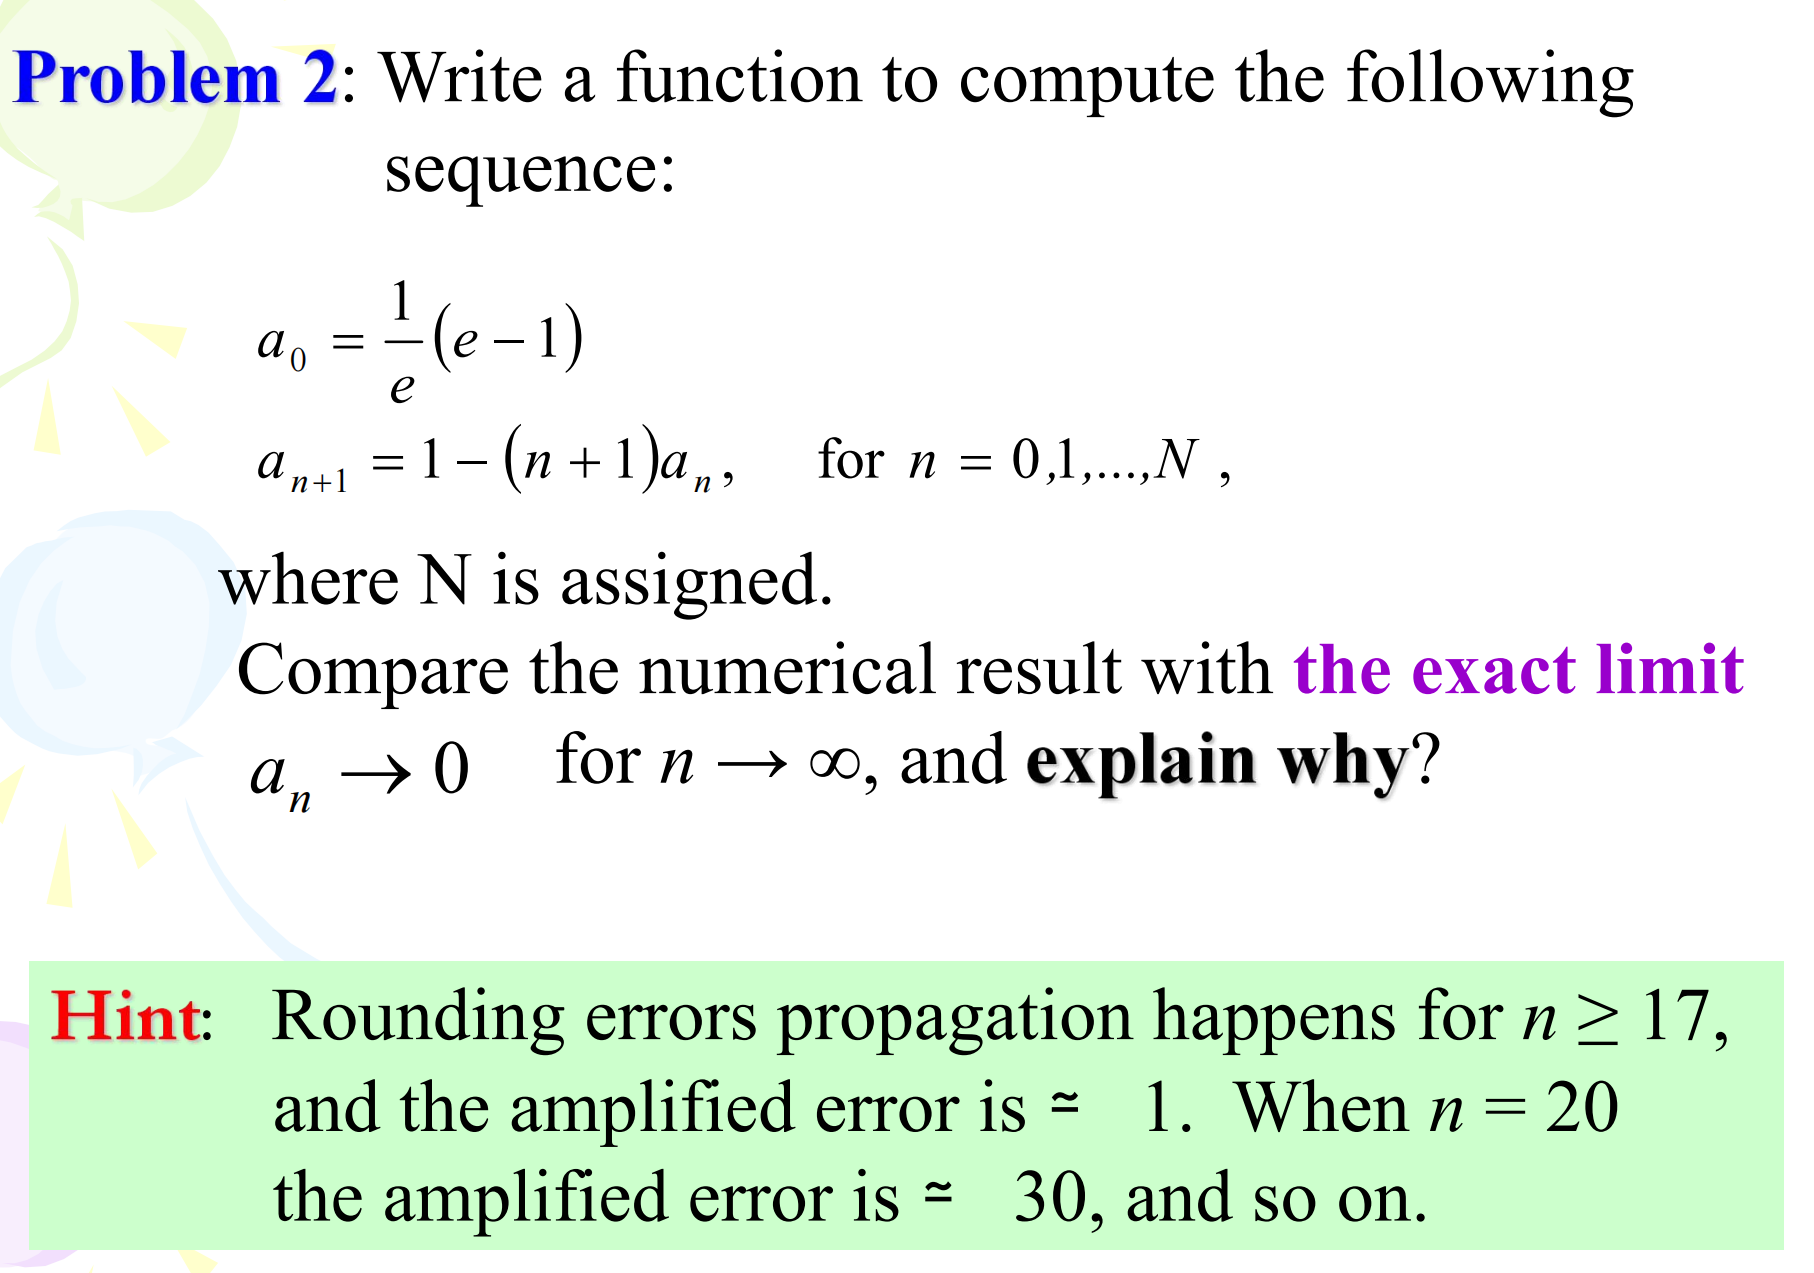
\includegraphics[width=0.7\textwidth]{pic/question.png}
\end{figure}

\newpage
\tableofcontents
\newpage

% =================================================
% Part 1
% =================================================
\section{Part 1. Source Code}

\begin{lstlisting}
#include <iostream>
#include <iomanip>
#include <cmath>
#include <vector>
#include <string>
#include <algorithm>
#include <cstdint>

using namespace std;

// ============================================================
// 理论值：a_n = ∫_0^1 x^n e^(x-1) dx
// 用 Simpson 积分
// ============================================================
long double exactValueIntegral(int n) {
    const int M = 200000;
    long double h = 1.0L / M;
    long double sum = 0.0L;

    for (int i = 0; i <= M; i++) {
        long double x = i * h;
        long double fx = powl(x, n) * expl(x - 1.0L);

        if (i == 0 || i == M)
            sum += fx;
        else if (i % 2 == 0)
            sum += 2.0L * fx;
        else
            sum += 4.0L * fx;
    }

    return sum * h / 3.0L;
}

// ============================================================
// 原程序真实递推（double）
// ============================================================
vector<double> computeRealRecursion(int N) {
    vector<double> a(N + 1);
    a[0] = (exp(1.0) - 1.0) / exp(1.0);

    for (int n = 0; n < N; ++n) {
        a[n + 1] = 1.0 - (n + 1) * a[n];
    }
    return a;
}

// ============================================================
// 非负大整数，base = 1e9
// ============================================================
struct BigUInt {
    static const uint32_t BASE = 1000000000U;
    vector<uint32_t> d; // little-endian

    void trim() {
        while (!d.empty() && d.back() == 0) d.pop_back();
    }

    bool isZero() const {
        return d.empty();
    }

    static BigUInt fromUint64(unsigned long long x) {
        BigUInt a;
        if (x == 0) return a;
        while (x) {
            a.d.push_back((uint32_t)(x % BASE));
            x /= BASE;
        }
        return a;
    }

    void mulSmall(uint32_t m) {
        if (isZero() || m == 0) {
            d.clear();
            return;
        }
        if (m == 1) return;

        unsigned long long carry = 0;
        for (size_t i = 0; i < d.size(); ++i) {
            unsigned long long cur = 1ULL * d[i] * m + carry;
            d[i] = (uint32_t)(cur % BASE);
            carry = cur / BASE;
        }
        while (carry) {
            d.push_back((uint32_t)(carry % BASE));
            carry /= BASE;
        }
    }

    uint32_t divSmall(uint32_t m) {
        unsigned long long rem = 0;
        for (int i = (int)d.size() - 1; i >= 0; --i) {
            unsigned long long cur = rem * BASE + d[i];
            d[i] = (uint32_t)(cur / m);
            rem = cur % m;
        }
        trim();
        return (uint32_t)rem;
    }

    string toDecimalString() const {
        if (isZero()) return "0";
        BigUInt tmp = *this;
        vector<uint32_t> parts;

        while (!tmp.isZero()) {
            parts.push_back(tmp.divSmall(BASE));
        }

        string s = to_string(parts.back());
        for (int i = (int)parts.size() - 2; i >= 0; --i) {
            string t = to_string(parts[i]);
            s += string(9 - t.size(), '0') + t;
        }
        return s;
    }

    // 仅用于显示近似值
    long double toLongDoubleApprox() const {
        if (isZero()) return 0.0L;

        string s = toDecimalString();
        int take = min((int)s.size(), 18);

        long double mant = 0.0L;
        for (int i = 0; i < take; ++i) {
            mant = mant * 10.0L + (s[i] - '0');
        }

        int exp10 = (int)s.size() - take;
        return mant * powl(10.0L, exp10);
    }
};

// ============================================================
// 有符号大整数
// ============================================================
struct SignedBigInt {
    int sign;   // -1, 0, +1
    BigUInt mag;

    SignedBigInt() : sign(0) {}

    bool isZero() const {
        return sign == 0 || mag.isZero();
    }

    static SignedBigInt fromScaledLongDouble(long double x, int SHIFT) {
        SignedBigInt a;
        if (x == 0.0L) return a;

        long double scaled = ldexpl(x, SHIFT);  // x * 2^SHIFT
        long double rounded = roundl(scaled);

        if (rounded == 0.0L) return a;

        a.sign = (rounded > 0.0L ? 1 : -1);
        unsigned long long v = (unsigned long long) llroundl(fabsl(rounded));
        a.mag = BigUInt::fromUint64(v);
        return a;
    }

    void mulSmallSigned(int k) {
        if (isZero() || k == 0) {
            sign = 0;
            mag.d.clear();
            return;
        }
        if (k < 0) {
            sign = -sign;
            k = -k;
        }
        mag.mulSmall((uint32_t)k);
        if (mag.isZero()) sign = 0;
    }

    // 仅用于显示近似值：先转 long double 再除 2^SHIFT
    long double toApproxError(int SHIFT) const {
        if (isZero()) return 0.0L;
        long double v = mag.toLongDoubleApprox();
        if (sign < 0) v = -v;
        return ldexpl(v, -SHIFT);
    }

    string toScientificString(int SHIFT, int sigDigits = 12) const {
        long double v = toApproxError(SHIFT);
        ostringstream oss;
        oss << scientific << setprecision(sigDigits) << v;
        return oss.str();
    }
};

int main() {
    int N;
    cout << "请输入 N: ";
    cin >> N;

    // 这个值可调：
    // M_n = round(e_n * 2^SHIFT)
    // SHIFT 越大，初值误差保留越细
    const int SHIFT = 80;

    // -----------------------------
    // 理论值
    // -----------------------------
    vector<long double> a_theory(N + 1);
    a_theory[0] = 1.0L - 1.0L / expl(1.0L);
    for (int n = 1; n <= N; ++n) {
        a_theory[n] = exactValueIntegral(n);
    }

    // -----------------------------
    // 原程序实际结果
    // -----------------------------
    vector<double> a_real = computeRealRecursion(N);

    vector<long double> real_err(N + 1);
    for (int n = 0; n <= N; ++n) {
        real_err[n] = (long double)a_real[n] - a_theory[n];
    }

    // -----------------------------
    // 误差模型：
    // e_n ≈ (-1)^n n! e0
    //
    // 这里 e0 取“原程序实际初值”与“理论初值”的差：
    // e0 = a0_real - a0_theory
    //
    // 内部不直接存 e_n，而存
    // M_n = round(e_n * 2^SHIFT)
    // 于是：
    // M_{n+1} = -(n+1) M_n
    // -----------------------------
    long double a0_theory = a_theory[0];
    double a0_real = a_real[0];
    long double e0 = (long double)a0_real - a0_theory;

    vector<SignedBigInt> pred(N + 1);
    pred[0] = SignedBigInt::fromScaledLongDouble(e0, SHIFT);

    for (int n = 0; n < N; ++n) {
        pred[n + 1] = pred[n];
        pred[n + 1].mulSmallSigned(-(n + 1));
    }

    // -----------------------------
    // Part 1
    // -----------------------------
    cout << "\n==================== Part 1 ====================\n";
    cout << "原程序递推值、理论值、真实误差\n\n";

    cout << scientific << setprecision(10);
    cout << setw(5)  << "n"
         << setw(20) << "a_n(real)"
         << setw(24) << "a_n(theory)"
         << setw(24) << "real_error"
         << "\n";

    for (int n = 0; n <= N; ++n) {
        cout << setw(5)  << n
             << setw(20) << a_real[n]
             << setw(24) << a_theory[n]
             << setw(24) << real_err[n]
             << "\n";
    }

    // -----------------------------
    // Part 2
    // -----------------------------
    cout << "\n==================== Part 2 ====================\n";
    cout << "误差模型：e_n ≈ (-1)^n n! e0\n";
    cout << "其中 e0 = a0_real - a0_theory\n";
    cout << "为了避免浮点爆炸，内部采用：\n";
    cout << "M_n = round(e_n * 2^SHIFT), SHIFT = " << SHIFT << "\n";
    cout << "然后精确递推：M_(n+1) = -(n+1) M_n\n";
    cout << "输出时再除以 2^SHIFT。\n\n";

    cout << scientific << setprecision(18);
    cout << "a0_theory = " << a0_theory << "\n";
    cout << "a0_real   = " << a0_real << "\n";
    cout << "e0        = " << e0 << "\n";
    cout << "pred[0]   = " << pred[0].toScientificString(SHIFT, 12) << "\n\n";

    cout << scientific << setprecision(10);
    cout << setw(5)  << "n"
         << setw(24) << "predicted_error"
         << "\n";

    for (int n = 0; n <= N; ++n) {
        cout << setw(5)  << n
             << setw(24) << pred[n].toApproxError(SHIFT)
             << "\n";
    }

    // -----------------------------
    // Part 3
    // -----------------------------
    cout << "\n==================== Part 3 ====================\n";
    cout << "将预测误差与真实误差比较\n\n";

    cout << setw(5)  << "n"
         << setw(24) << "real_error"
         << setw(24) << "predicted_error"
         << setw(24) << "difference"
         << "\n";

    for (int n = 0; n <= N; ++n) {
        long double est = pred[n].toApproxError(SHIFT);
        long double diff = real_err[n] - est;

        cout << setw(5)  << n
             << setw(24) << real_err[n]
             << setw(24) << est
             << setw(24) << diff
             << "\n";
    }

    return 0;
}
\end{lstlisting}

% =================================================
% Part 2
% =================================================
\section{Part 2. Basic Principles}

This program studies the sequence
\begin{equation}
    a_0 = 1 - \frac{1}{e},
\end{equation}
and
\begin{equation}
    a_{n+1} = 1 - (n+1)a_n, \qquad n = 0,1,2,\dots,N.
\end{equation}
The main purpose is not only to compute the recurrence numerically, but also to compare the direct floating-point recursion with the theoretical behavior of the exact sequence and with a separate prediction of the propagated round-off error.

\subsection*{Mathematical Background}

A useful exact representation of the sequence is
\begin{equation}
    a_n = \int_0^1 x^n e^{x-1} \, dx.
\end{equation}
By integration by parts,
\begin{equation}
    \int_0^1 x^{n+1} e^{x-1} \, dx
    = \left[x^{n+1} e^{x-1}\right]_0^1 - (n+1)\int_0^1 x^n e^{x-1} \, dx,
\end{equation}
so we obtain
\begin{equation}
    a_{n+1} = 1 - (n+1)a_n.
\end{equation}
Therefore the recurrence in the assignment is fully consistent with the integral formula used in the program.

The exact limit is
\begin{equation}
    a_n \to 0 \qquad (n \to \infty),
\end{equation}
because for $x \in [0,1]$ we have $0 \le e^{x-1} \le 1$ and hence
\begin{equation}
    0 \le a_n = \int_0^1 x^n e^{x-1} \, dx \le \int_0^1 x^n \, dx = \frac{1}{n+1} \to 0.
\end{equation}
However, the direct forward recursion is numerically unstable, so the computed values in finite precision may eventually depart completely from the true limit.

\subsection*{Methodology}

The submitted C++ program contains three logically different computations.

\begin{enumerate}[label=\arabic*.]
    \item \textbf{Direct recursion in double precision.} \\
    The function \texttt{computeRealRecursion(int N)} stores the sequence in a \texttt{vector<double>} and computes
    \begin{equation}
        a_{n+1}^{(\mathrm{real})} = 1 - (n+1)a_n^{(\mathrm{real})}.
    \end{equation}
    This part reproduces the straightforward algorithm that one would naturally write first.

    \item \textbf{Reference values from numerical quadrature.} \\
    In order to compare the floating-point result with a much more reliable reference, the function \texttt{exactValueIntegral(int n)} evaluates
    \begin{equation}
        a_n^{(\mathrm{theory})} = \int_0^1 x^n e^{x-1} \, dx
    \end{equation}
    by composite Simpson integration with $M = 200000$ subintervals and the type \texttt{long double}. This is a distinctive feature of the code: instead of using the same recurrence for the reference solution, the program constructs the theoretical value independently from the integral formula, which avoids circular verification.

    \item \textbf{Explicit error propagation model.} \\
    Let
    \begin{equation}
        e_n = a_n^{(\mathrm{real})} - a_n.
    \end{equation}
    If we temporarily ignore the newly generated round-off term at each step, then the recurrence implies
    \begin{equation}
        e_{n+1} \approx -(n+1)e_n,
    \end{equation}
    and therefore
    \begin{equation}
        e_n \approx (-1)^n n! e_0.
    \end{equation}
    The program implements this model separately and prints the predicted error together with the actual error.
\end{enumerate}

\subsection*{Special Design of the Program}

The most interesting part of the implementation is the way the error model is stored. Since the quantity $(-1)^n n! e_0$ grows extremely fast, it would soon overflow if it were propagated directly as a standard floating-point number. To avoid this problem, the program defines two custom integer types:
\begin{itemize}
    \item \texttt{BigUInt}: a nonnegative big integer with base $10^9$;
    \item \texttt{SignedBigInt}: a signed wrapper built on top of \texttt{BigUInt}.
\end{itemize}

Instead of storing $e_n$ itself, the code stores a scaled integer
\begin{equation}
    M_n = \mathrm{round}(e_n 2^{\texttt{SHIFT}}), \qquad \texttt{SHIFT}=80.
\end{equation}
Then the error model is propagated by the exact integer recursion
\begin{equation}
    M_{n+1} = -(n+1)M_n.
\end{equation}
Only when the result is printed does the program convert back by dividing by $2^{\texttt{SHIFT}}$. This design is very suitable for the present homework, because it preserves the amplification law of the error without introducing additional instability into the prediction itself.

\subsection*{Program Flow}

The complete workflow of the program can be summarized as follows:
\begin{enumerate}[label=\arabic*.]
    \item read the assigned integer $N$;
    \item compute $a_n^{(\mathrm{theory})}$ from the integral representation using Simpson's rule;
    \item compute $a_n^{(\mathrm{real})}$ by the original forward recurrence in \texttt{double};
    \item evaluate the true error
    \begin{equation}
        \mathrm{real\_err}_n = a_n^{(\mathrm{real})} - a_n^{(\mathrm{theory})};
    \end{equation}
    \item construct the predicted error sequence from $e_0$ using the scaled big-integer recursion;
    \item print three parts of output: direct results, predicted error, and comparison between the two.
\end{enumerate}

The computational cost of the direct recurrence is $O(N)$, while the cost of generating the theoretical reference is dominated by the numerical integration. Since the quadrature uses a fixed large number of subintervals, the program favors reliability of comparison over raw efficiency, which is a reasonable choice for this report-style assignment.

% =================================================
% Part 3
% =================================================
\section{Part 3. Displayed Results}

This section presents representative outputs obtained from the submitted program with input $N=30$.

\subsection*{Representative Terminal Output}

The first part of the program prints the recursively computed values, the reference values obtained from the integral, and the true error. A typical excerpt is listed below.

\begin{lstlisting}
Input N = 30

n    a_n(real)          a_n(theory)        real_error
16   5.5459301730e-02   5.5719345931e-02  -2.6004420167e-04
17   5.7191870597e-02   5.2771119169e-02   4.4207514283e-03
18  -2.9453670752e-02   5.0119854958e-02  -7.9573525710e-02
19   1.5596197443e+00   4.7722755796e-02   1.5118969885e+00
20  -3.0192394886e+01   4.5544884076e-02  -3.0237939770e+01
\end{lstlisting}

The table clearly shows that the direct recursion is still reasonable for small $n$, but around $n=17$ the error starts to grow rapidly, and by $n=20$ the computed value has completely lost the correct magnitude and sign.

\subsection*{Observed Numerical Results}

Table~\ref{tab:key-results} summarizes several representative values extracted from the program output. The selected rows highlight the transition from a stable-looking phase to a catastrophic error-amplification phase.

\begin{table}[H]
    \centering
    \caption{Representative numerical results for $N=30$}
    \label{tab:key-results}
    \begin{tabular}{cccc}
        \toprule
        $n$ & $a_n^{(\mathrm{real})}$ & $a_n^{(\mathrm{theory})}$ & $a_n^{(\mathrm{real})} - a_n^{(\mathrm{theory})}$ \\
        \midrule
        10 & $8.3877070058\times10^{-2}$ & $8.3877070103\times10^{-2}$ & $-4.5101461377\times10^{-11}$ \\
        15 & $5.9033793642\times10^{-2}$ & $5.9017540879\times10^{-2}$ & $1.6252762604\times10^{-5}$ \\
        17 & $5.7191870597\times10^{-2}$ & $5.2771119169\times10^{-2}$ & $4.4207514283\times10^{-3}$ \\
        18 & $-2.9453670752\times10^{-2}$ & $5.0119854958\times10^{-2}$ & $-7.9573525710\times10^{-2}$ \\
        20 & $-3.0192394886\times10^{1}$ & $4.5544884076\times10^{-2}$ & $-3.0237939770\times10^{1}$ \\
        25 & $1.9278500883\times10^{8}$ & $3.7086214424\times10^{-2}$ & $1.9278500880\times10^{8}$ \\
        30 & $-3.2967624556\times10^{15}$ & $3.1279673932\times10^{-2}$ & $-3.2967624556\times10^{15}$ \\
        \bottomrule
    \end{tabular}
\end{table}

The exact sequence decreases slowly toward zero, whereas the directly computed sequence eventually oscillates with enormous amplitude. This behavior is the main numerical phenomenon that the homework asks us to explain.

\subsection*{Error Prediction Output}

The second part of the code prints the predicted error generated from
\begin{equation}
    e_n \approx (-1)^n n! e_0.
\end{equation}
For the present run, the initial error is approximately
\begin{equation}
    e_0 = a_0^{(\mathrm{real})} - a_0^{(\mathrm{theory})} \approx -1.2468\times 10^{-17}.
\end{equation}
Although this number is tiny, multiplication by $n!$ makes it dominant after only a moderate number of steps. For example, the predicted error is already of order $10^{-1}$ near $n=18$, of order $10^1$ near $n=20$, and becomes astronomically large afterwards. This is consistent with the actual behavior observed in the direct recursion.

\subsection*{Program Screenshots}

The following pictures show the output of the program, with N inputted 30.

\begin{figure}[H]
    \centering
    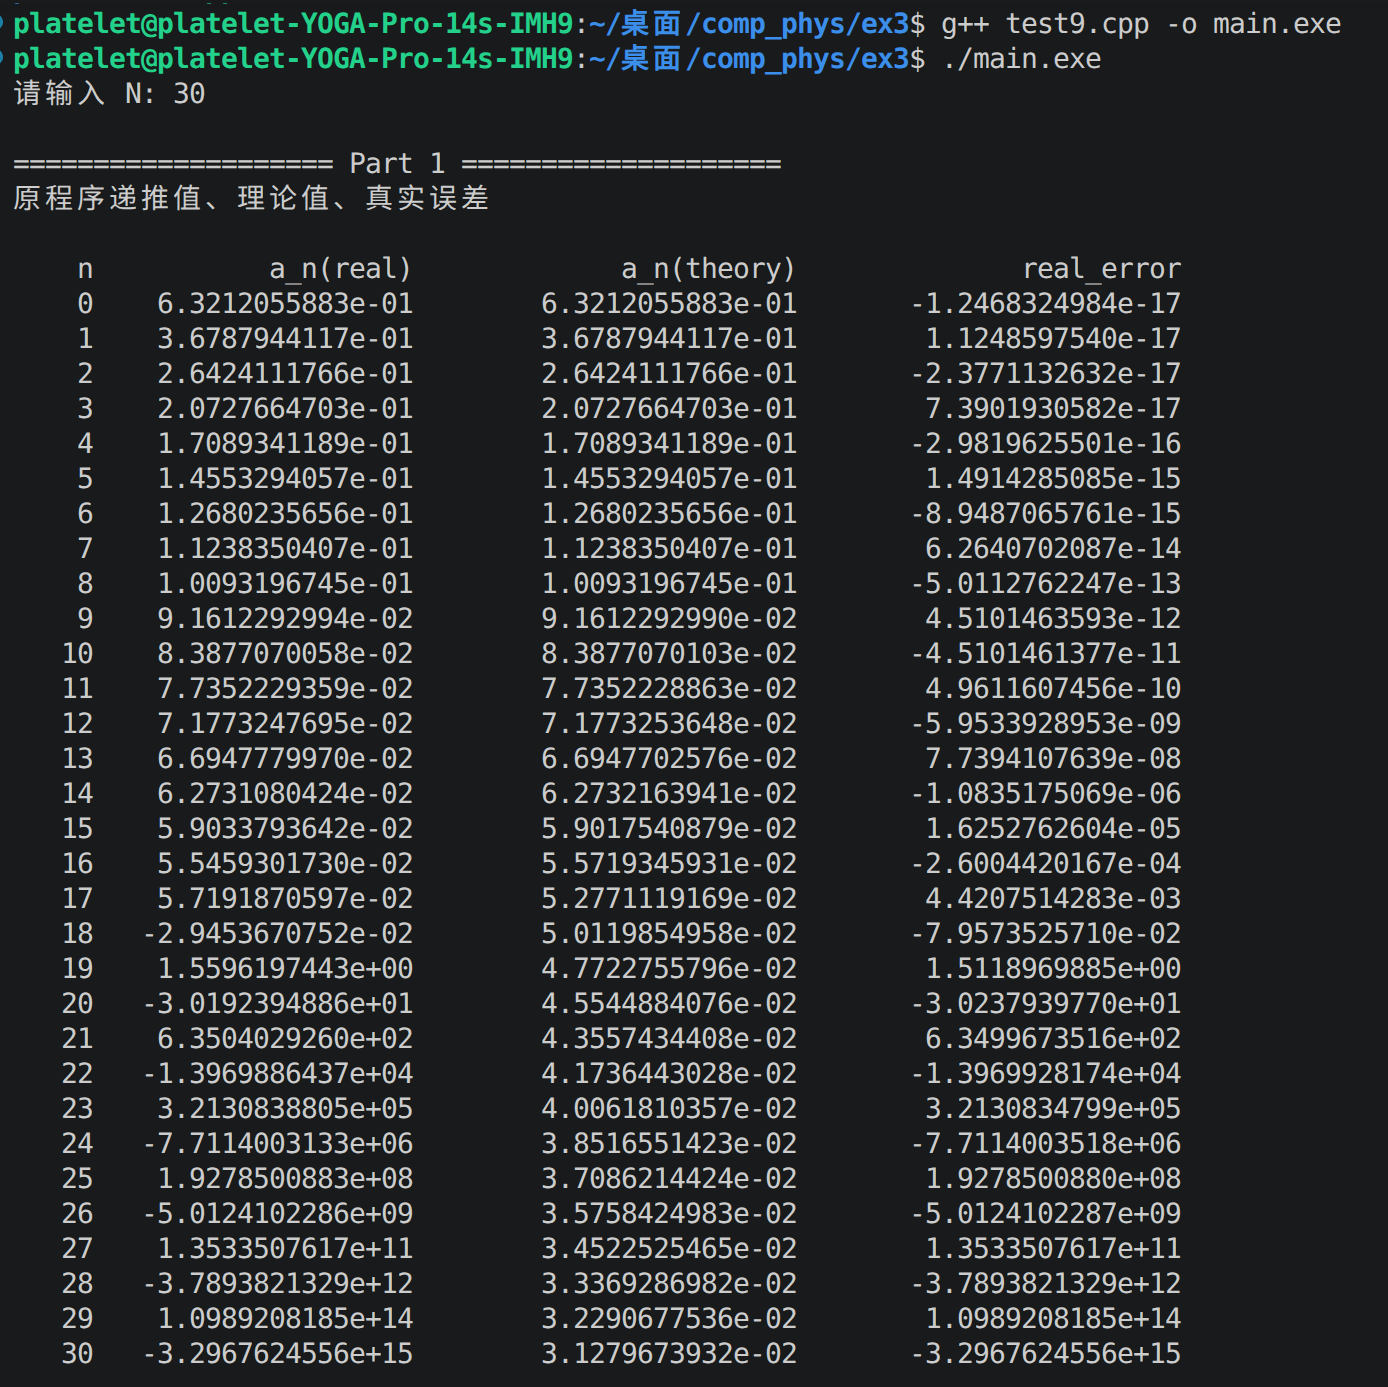
\includegraphics[width=0.95\textwidth]{pic/ans1.png}
    \label{fig:part1-output}
\end{figure}

\begin{figure}[H]
    \centering
    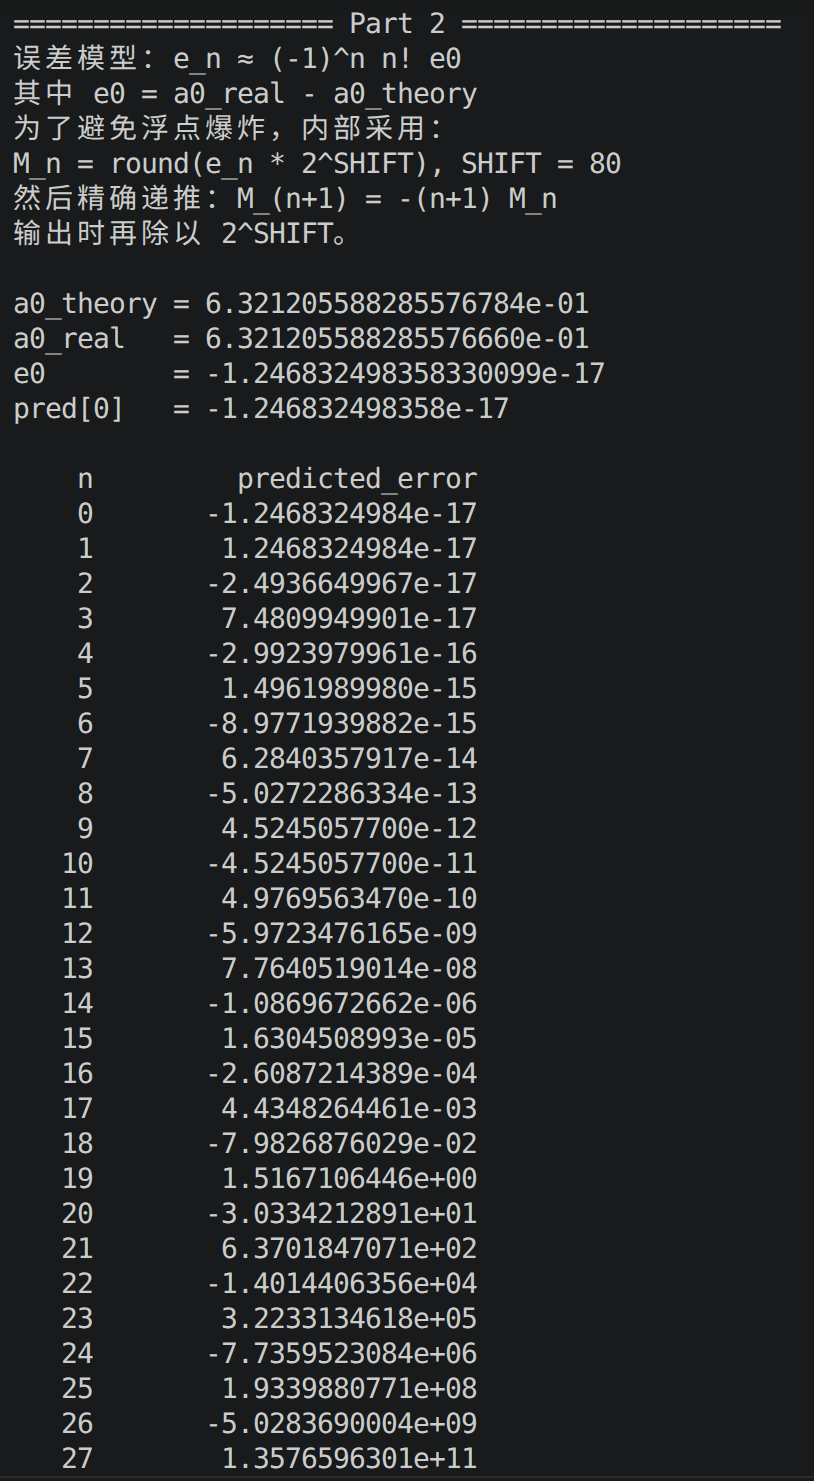
\includegraphics[width=0.72\textwidth]{pic/ans2.png}
    \label{fig:part2-output}
\end{figure}

\begin{figure}[H]
    \centering
    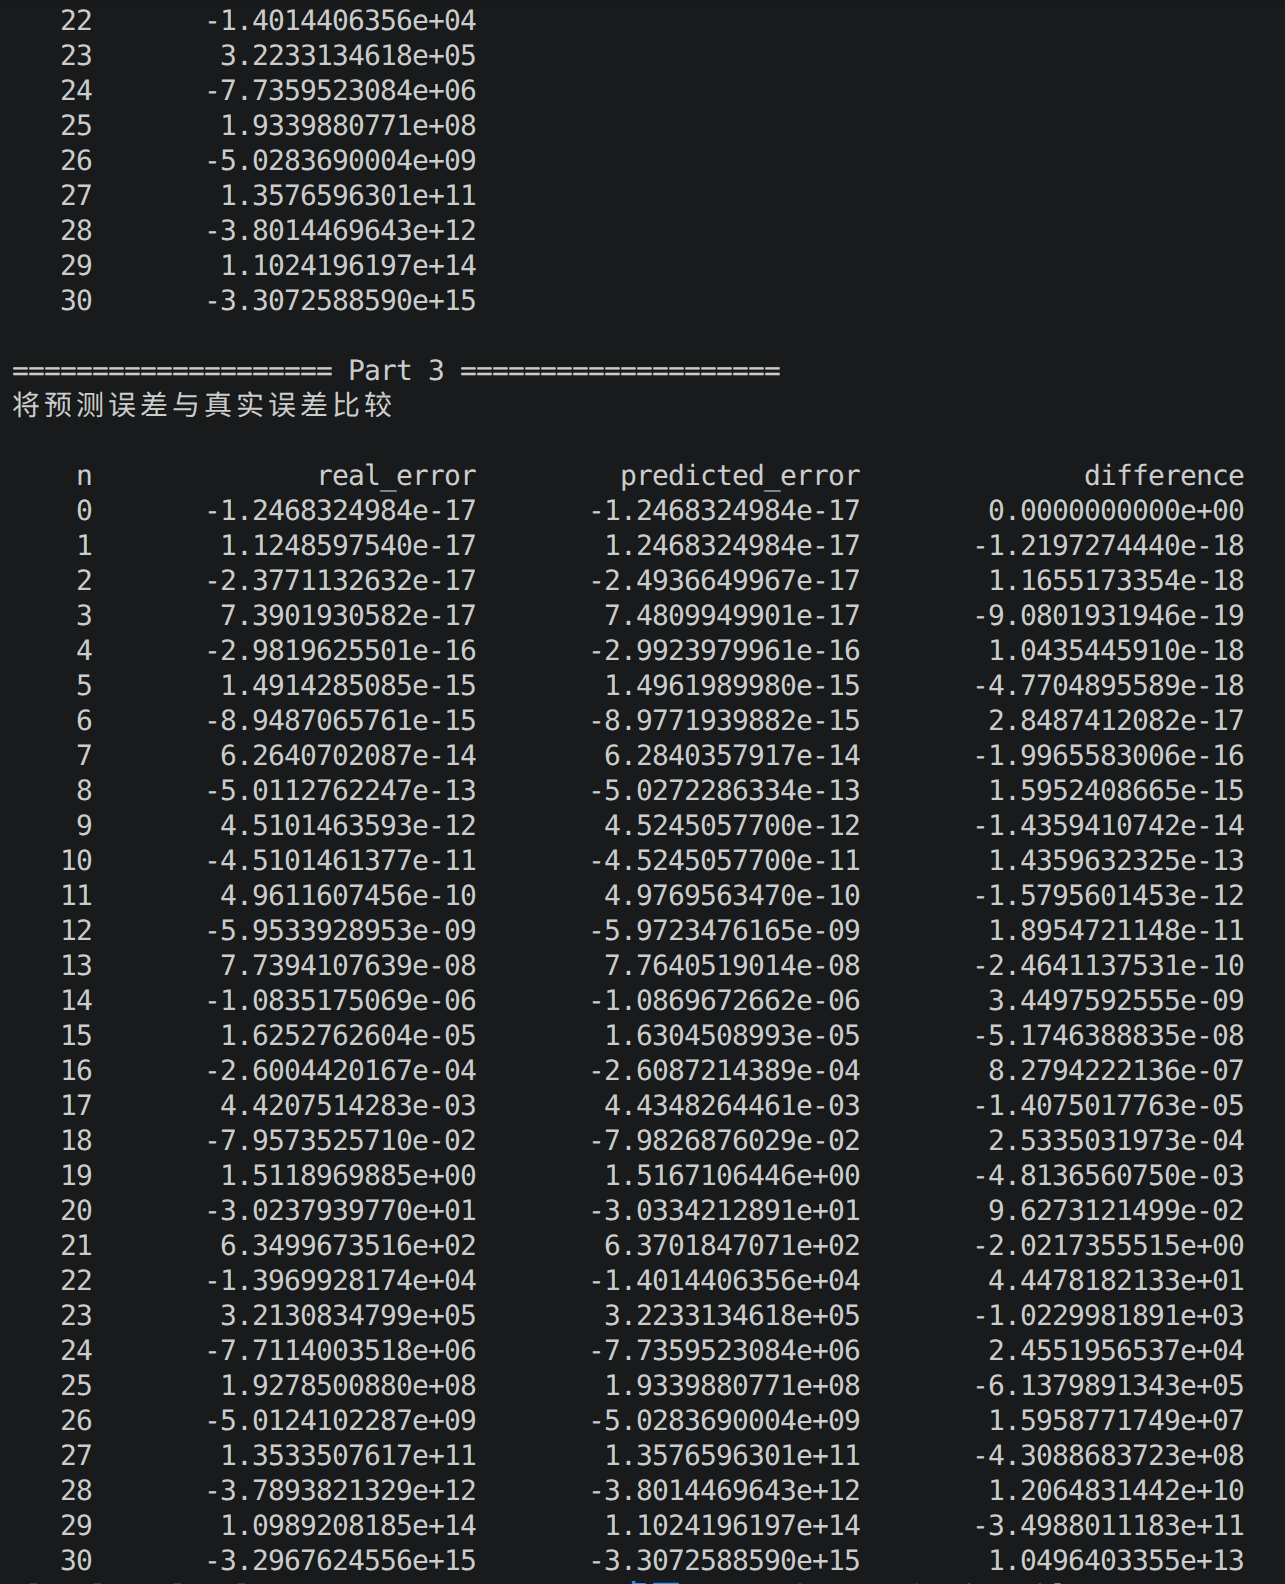
\includegraphics[width=0.72\textwidth]{pic/ans3.png}
    \label{fig:part3-output}
\end{figure}

% =================================================
% Part 4
% =================================================
\section{Part 4. Discussion}

\subsection*{Interpretation of Results}

The numerical results show two very different facts at the same time.

First, the \emph{exact} sequence is perfectly well-behaved. Since $a_n$ has the integral representation
\begin{equation}
    a_n = \int_0^1 x^n e^{x-1} \, dx,
\end{equation}
it remains positive and decreases toward zero. The theoretical column in the output confirms this: for $n=30$ the value is still about $3.13\times10^{-2}$, so the decay is relatively slow but completely regular.

Second, the \emph{direct floating-point recurrence} is extremely sensitive to perturbations. Once the accumulated error reaches a visible level, the recurrence multiplies it by the factor $-(n+1)$ at the next step. Because this factor grows linearly with $n$, the total amplification behaves essentially like a factorial. As a result, a harmless machine-level perturbation at the beginning becomes the dominant contribution later, and the computed sequence no longer reflects the true mathematics of the problem.

\subsection*{Why the Forward Recurrence Fails}

Suppose the computed value is
\begin{equation}
    \widetilde{a}_n = a_n + e_n.
\end{equation}
Substituting this into the recurrence gives
\begin{equation}
    \widetilde{a}_{n+1} = 1 - (n+1)\widetilde{a}_n,
\end{equation}
while the exact value satisfies
\begin{equation}
    a_{n+1} = 1 - (n+1)a_n.
\end{equation}
Subtracting the two equations yields
\begin{equation}
    e_{n+1} = -(n+1)e_n + \delta_n,
\end{equation}
where $\delta_n$ denotes the new round-off introduced at step $n$. If the propagated part dominates $\delta_n$, then
\begin{equation}
    e_n \approx (-1)^n n! e_0.
\end{equation}
This is exactly the law implemented in the prediction module of the program. The numerical output confirms that this model captures the growth rate and sign alternation of the real error very well once the instability starts to dominate.

Another intuitive explanation is cancellation. For moderate $n$, the exact product $(n+1)a_n$ is close to $1$. Therefore the recurrence computes $a_{n+1}$ as the difference of two nearly equal numbers,
\begin{equation}
    a_{n+1} = 1 - (n+1)a_n,
\end{equation}
which is a classical setting in which significant digits are lost. After that loss of precision occurs, the next multiplication by $(n+1)$ magnifies the remaining error. Hence the recurrence is not backward stable in finite precision arithmetic.

\subsection*{Error Analysis and Prediction}

The output of the program provides a clear quantitative picture of the error growth.
\begin{itemize}
    \item For small $n$, the error remains close to machine precision and the direct recursion appears trustworthy.
    \item Around $n=15$ to $17$, the error becomes visible on the scale of the exact answer.
    \item Near $n=18$ to $20$, the propagated error exceeds the exact value itself, so the numerical result changes sign and then explodes in magnitude.
    \item After that point, the computed sequence is almost entirely an error-propagation process rather than an approximation to $a_n$.
\end{itemize}

The prediction part of the code is especially valuable because it does not merely state that ``round-off error exists''; instead, it models the mechanism explicitly. Since the program stores the predicted error in the form
\begin{equation}
    M_n = \mathrm{round}(e_n 2^{80}),
\end{equation}
it can continue tracking the factorial amplification without suffering from the same overflow and precision loss that affect the original recursion. Therefore the comparison between the true error and the predicted error gives strong evidence that the blow-up is caused primarily by the recurrence itself, not by the quadrature reference.

A small discrepancy remains between the predicted and observed errors. This is expected, because the simplified model keeps only the amplified initial perturbation $e_0$ and does not include every local round-off term $\delta_n$ generated along the way. Nevertheless, once the instability dominates, the leading-order model is already sufficient to explain the overall magnitude and alternating sign pattern.

\vfill
\begin{center}
    \textit{End of Report}
\end{center}

\end{document}